\chapter{Propagação incerteza}

\vspace{-0.7cm}

\begin{num}

\item Os lados de um paralelepípedo são $a$ = (4,50 $\pm$ 0,05) cm, $b$ = (8,50 $\pm$ 0,09)~cm e $c$ = (35,0 $\pm$ 0,3) mm. Determinar o volume do cubo com sua incerteza absoluta e relativa.

\item Na medição da resistência (R), se obteve o valor da tensão V = (15,2 $\pm$ 0,2)~V e da corrente I = (2,6 $\pm$ 0,1)~A. Qual é a incerteza absoluta da resistência usando a equação R = V/I?
 
\item Um pêndulo simples é utilizado para medir o valor da aceleração da gravidade utilizando equação:

\[ 
T = 2 \pi \sqrt{\frac{l}{g}}.
\]
\noindent
O período $T$ medido foi de (1,24 $\pm$ 0,02)~s e o comprimento do pêndulo $l$ = (0,381 $\pm$ 0,002)~m. Qual é o resultado do valor da aceleração da gravidade $g$ com sua incerteza absoluta e relativa?

\item Para medir o comprimento total de um pêndulo (fio + esfera) usou-se uma régua milimetrada para medir o comprimento do fio e um paquímetro para medir o diâmetro da esfera. Observam-se os seguintes valores com as suas respectivas incertezas: 
\begin{iten}
\item[ ]Comprimento do fio = 2,100 m			
\item[ ] Incerteza comprimento do fio = 0,5 cm
\item[ ]Diâmetro da esfera = 2,114 cm			
\item[ ] Incerteza do diâmetro da esfera = 0,01 mm
\end{iten}
\noindent 
Ache o comprimento total e a sua incerteza associada.

\item Para o cálculo do volume de uma esfera, foi dado o raio da mesma: R = (232,0 $\pm$ 0,1)~mm. Calcular seu volume com a sua respectiva incerteza relativa.

\item A partir da figura~\ref{fig:fig1}, com as seguintes medidas:
\begin{iten}
\item[ ] L1 = (5,00 $\pm$ 0,05) cm
\item[ ] L2 = (20,00 $\pm$ 0,05) mm
\item[ ] L3 = (15,00 $\pm$ 0,01) mm
\end{iten}
\begin{figure}[t]
\begin{center}
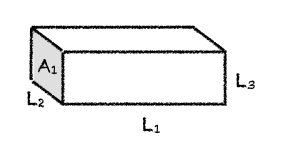
\includegraphics[width=8cm]{fig/Fig1}
\caption{\label{fig:fig1} Bloco retangular.}
\vspace{-0.4cm}
\end{center}
\end{figure}
\begin{num}
\item Determine a área A1 com a incerteza correspondente.
\item Determine o volume desta peça com a incerteza correspondente.
\item Se a precisão necessária para o resultado da área é de 0,5\% podemos considerar este resultado satisfatório?
\end{num}

\item Para determinar a altura de uma cachoeira, algumas pessoas mediram o tempo de queda de pedrinhas que eram soltas, em queda livre, de um mesmo local. Conhecendo o tempo de queda $t$, pode-se calcular a altura $h$ a partir da relação cinemática $h = 1/2 g t^2$ em que $g$ é a aceleração da gravidade. Foi utilizado um cronômetro com precisão de centésimos de segundo e os valores $t_i$ obtidos em 8 medidas estão na seguinte tabela:

\begin{center}
  \begin{tabular}{|>{ \centering\arraybackslash}m{1cm}  |>{ \centering\arraybackslash}m{2cm} |}  \hline
    	& t(s)	 \\ \hline	 	
  1	& 1,30\\ \hline	 
2	&1,09\\ \hline	 
3	&1,03\\ \hline	 
4	&1,27\\ \hline	 
5	&1,18\\ \hline	 
6	&1,31\\ \hline	 
7	&1,24\\ \hline	 
8	&1,15\\ \hline	 
  \end{tabular}
  \end{center}

Considerando $g = (9,784 \pm 0,001)$~m/s$^2$, calcule a altura da cachoeira e a sua incerteza.

\end{num}
